\section{Conclusiones}
\begin{frame}
	\frametitle{Conclusiones}
	\begin{figure}
	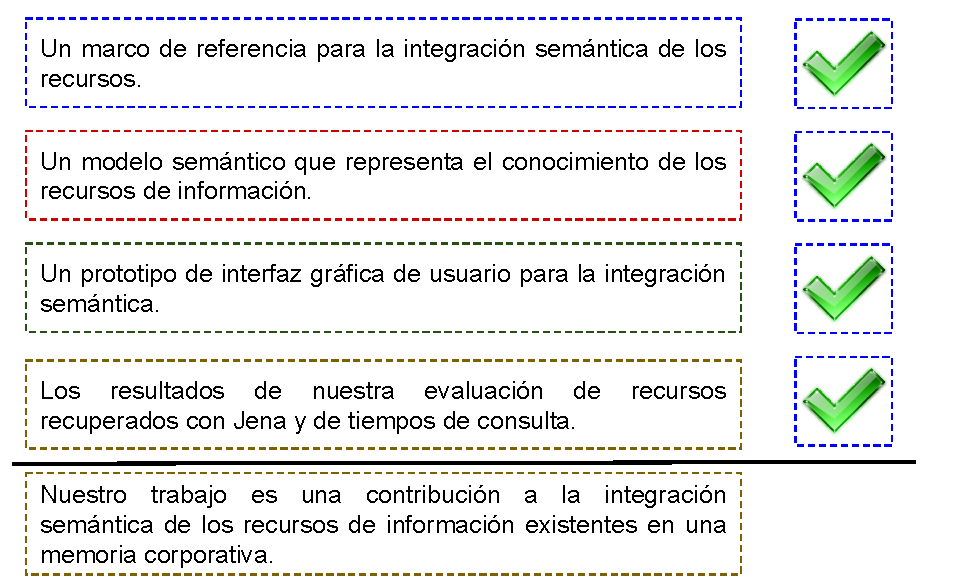
\includegraphics[scale=0.6]{ConclusionesObj} 
	\end{figure}
\end{frame}

\begin{frame}
	\frametitle{Conclusiones}
	\begin{exampleblock}{Hip�tesis}
	\justifying 
	\textbf{El uso de las \textit{tecnolog�as sem�nticas} es adecuado para lograr la \textit{integraci�n sem�ntica} de \textit{recursos de informaci�n} en una \textit{memoria corporativa}}.
	\end{exampleblock}
	
	\begin{block}{Ventajas de las Tecnolog�as Sem�nticas}
	\begin{itemize}
	\item \justifying Modelos en un formato est�ndar.
	\item \justifying Modelos flexibles, extensibles y reutilizables.
	\item \justifying Uso de Lenguajes est�ndar (World Wide Web Consortium).
	\item \justifying Modelos con conocimiento expl�cito e impl�cito.
	\item \justifying Inferencia para materializar tripletas RDF.
	\item \justifying Aplicaciones gen�ricas.
	\end{itemize}
	\end{block}
\end{frame}

\begin{frame}
	\frametitle{Recomendaciones}
	\begin{block}{}
	\begin{itemize}
	\item \justifying \small Modulo para la generaci�n de descripciones sem�nticas de los \textit{recursos de informaci�n}.
		\begin{itemize}
		\item \justifying \small Autom�tica mediante \textit{miner�a de texto}.
		\item \justifying \small Generaci�n manual de descripciones, mediante la escritura de informaci�n por un usuario.
		\end{itemize}
	\end{itemize}
	\item \justifying \small 
	\end{block}
\end{frame}